\chapter{Avaliação e análise de desempenho}

\section{Introdução}

Após a definição da estrutura da arquitetura de referência SOA, que utiliza serviços web \emph{RESTfull}, conforme apresentado no capítulo~\ref{cap:Protocolo},  e onde foi proposto um protocolo de autenticação e autorização que tem por finalidade prover segurança a essa arquitetura, optou-se por realizar uma an\'{a}lise de seguran\c ca e experimentos que possibilitam a mensuração do impacto da sua utilização na infraestrutura da PCDF. Desta forma, este capítulo apresenta a avaliação da proposta descrita na disserta\c c\~{a}o.

\section{Análise de Segurança}

Nesta seção serão discutidas as propriedades de segurança do protocolo de autenticação e autorização proposto. São abordadas as propriedades e alguns ataques que podem ser realizados contra ele. Essa seção segue o padrão determinado no trabalho~\cite{traust08}.

\subsection{Segurança da sessão}

O protocolo de Autenticação e Autorização proposto utiliza para segurança de seção e da camada de transporte, o protocolo TLS/SSL. A utilização desse protocolo tem por objetivo evitar o ataque man-in-the-middle. Para isso, é exigido tanto do órgão conveniado como da própria PCDF que ambas utilizem certificados digitais padrão X.509 emitidos e garantidos por uma AC que esteja subordinada à hierarquia da ICP-Brasil.

Com isso, ambas as partes envolvidas no processo de comunicação podem estabelecer um processo de confiança mútua no nível de transporte. Todo o tráfego que flui sobre uma sessão bilateral certificada tem uma fonte confiável. Isso permite que implementações de serviços possam autorizar ou desautorizar interações com base na fonte bem conhecida de uma solicitação HTTP.

Além da segurança oferecida pela utilização da segurança na camada de transporte, com utilização do TLS/SSL, o protocolo utiliza mecanismos de segurança tais como criptografia assimétrica e assinatura digital. Isso Permite que outras partes mal intencionadas não consigam ter acesso ao conteúdo das mensagens trocadas pelo protocolo no processo de comunicação.

Diferentemente do sistema Traust, o protocolo de Autenticação e Autorização proposto, não será executado em ambientes em que nem o cliente nem o servidor tem uma chave pública certificada, procura-se dessa forma, atenuar problemas relacionados ao protocolo TLS, que quando executado em ambientes em que nem o cliente nem o servidor tem uma chave pública certificada, pode ser vulnerável a um ataque man-in-the-middle durante o estabelecimento da sessão~\cite{traust08}.

\subsection{Responsabilização dos usuários conveniados}

Uma das ameaças verificadas diz respeito a possibilidade do uso indevido, por parte dos órgãos conveniados, das informações disponibilizadas nos serviços ofertados pela PCDF. Isso decorre do fato das informações disponibilizadas serem sensíveis e possuírem caráter sigiloso. Dessa forma, para evitar esse problema é exigido dos órgãos conveniados que assinem um contrato para o consumo do serviço. No momento da assinatura do contrato eles recebem uma tabela contendo várias credenciais que servem como identidades e que deverão ser utilizadas no processo de autenticação, conforme descrito no seção~\ref{sec:reqprotocolo}. Isso possibilita que haja uma autenticação mútua entre a PCDF e os consumidores dos serviços. Além disso, com a utilização do protocolo de autenticação e autorização proposto, são empregados mecanismos de criptografia e assinaturas digitais que são geradas a partir de certificados digitais padrão X.509 vinculados aos órgãos e garantidos por AC. Dessa forma, busca-se evitar o não-repúdio por parte dos órgãos conveniados, atribuindo-lhes responsabilidades em caso do mau uso dos serviço ofertados pela PCDF.

Logo, uma vez detectado algum tipo de vazamento de dados proveniente dos serviços ofertados o órgão poderá ser identificado e após uma apuração minuciosa, responsabilizado pelos danos causados à PCDF.

\subsection{Ataques de repetição}
Esta ameaça, conforme descrito no capitulo~\ref{cap:revisaolit}, seção~\ref{sec:vulnerabilidadessoa}, se empregada contra o protocolo de autenticação e autorização proposto, tem uma chance quase nula de sucesso. Uma vez que são empregados \emph{timestamps} em em todas as trocas de mensagens realizadas pelo protocolo. Além disso, são gerados números únicos, que identificam os desafios de autenticação gerados e podem ser utilizados como \emph{nonces}, que também podem ser empregados contra esse tipo de ataque.

\subsection{Ataques de negação de serviço}

Esta ameaça é muito difícil de ser evitada, haja vista que,  pode ser fruto de ataques via rede, do consumo excessivo de recursos da máquina,  ou ainda,  ser resultante da exploração de qualquer tipo de vulnerabilidade que implique na indisponibilidade do serviço ou de um recurso. O protocolo de autenticação e autorização proposto é baseado no esquema de desafio-resposta. Os desafios são gerados de forma aleatória a partir das credenciais que identificam unicamente os consumidores dos serviços, o que possibilita uma autenticação mútua. Além disso, também são empregados outros mecanismos de segurança como utilização da segurança na camada de transporte e mecanismos de criptografia e assinaturas digitais. Isso minimiza a ameaça de ataques de negação de serviço.

Assim como o sistema Traust,~\cite{traust08}, o servidor de autenticação e autorização proposto pode ser replicado para outros servidores, o que possibilita um balanceamento de carga e minimiza a criação de gargalos. Isso permite que o servidor de autenticação seja escalável e esteja disponível em situações críticas, como no caso dos ataques de negação de serviço.


\subsection{Roubo de credenciais de autenticação e autorização}\label{subsec:RouboCred}

O protocolo de autenticação a autorização proposto após executado corretamente emite um token de segurança que será utilizado para a obtenção do serviço desejado, conforme apresenato na seção~\ref{sec:ArqProtocolo}, cabe ressaltar que se por algum motivo um atacante, conseguir burlar o os mecanismos de segurança utilizados pelo protocolo e conseguir acesso a essa credencial de autenticação e autorização ele terá acesso apenas um serviço, pois o protocolo emite credenciais para um único serviço por vez e com tempo de expiração determinado no momento de sua geração.

Essa é uma situação muito difícil de ser verificada, porém caso ocorra o problema é minimizado e não terá grande impacto na arquitetura do protocolo como um todo.

Outro problema que pode ocorrer é o roubo de credenciais de autenticação, que são as credenciais que o órgão conveniado recebe no momento da assinatura do contrato de oferecimento do serviço. Essa credenciais são utilizadas para responder os desafios que serão realizadas pelo protocolo de autenticação proposto. Caso isso ocorra e seja identificado a PCDF pode de forma rápida e transparente desativar as credenciais que julgar que foram comprometidas sem que o usuário seja prejudicado. Em um caso mais extremo, outras podem ser geradas e redistribuíras ao órgão conveniado.

Porém cabe ressaltar que caso ocorra o roubo de credenciais, o órgão que teve o problema será investigado e poderá ser responsabilizado se for detectado má fé má gestão na guarda das credenciais, conforme descrito na subseção~\ref{subsec:RouboCred}


\subsection{Ponto único de ataque}

Uma das possibilidades verificadas é que ocorrendo um ataque, o alvo possa não ser protocolo de autenticação e autorização proposto e sim o próprio servidor de autenticação e autorização. Neste caso, se o atacante for bem sucedido em sua empreitada o servidor poder ficar vulnerável. Esse servidor é responsável pela geração dos desafios de autenticação e pela geração das credenciais de autenticação e autorização. Porém, apesar de realizar estas atividades ele armazena e consulta os dados gerados no processo de autenticação e autorização em outra máquina, que é em um servidor de banco de dados. Em outras palavras o servidor de autenticação e autorização está em uma máquina diferente do servidor de banco de dados, o que minimiza os problemas relacionados a esse tipo de ataque, pois o servidor pode ser replicado para outra máquina e o que estiver com problemas pode ser fácilmente substituído.

\section{Testes de desempenho}

Testes de desempenho são definidos como uma investigação técnica realizada para determinar a capacidade de resposta, produtividade, confiabilidade e ou escalabilidade de um sistema, sob uma determinada carga de trabalho~\cite{Meier2007}.
A análise de desempenho possibilita identificar problemas que geralmente são encontrados em sistemas computacionais. Esses problemas podem ser agrupados em tópicos de: comparação e configuração de sistemas, identificação de gargalos, caracterização de cargas de trabalho e a previsão de desempenho~\cite{jain1991art}. Sendo assim, a análise de desempenho do protocolo de autenticação e autorização proposto foi dividida em dois estudos de caso que são apresentados nas seções~\ref{sec:caso1} e ~\ref{sec:caso2}.

\section{Estudo de caso 1}\label{sec:caso1}

Nesta seção será apresentada a metodologia empregada para a realização do teste de desempenho bem como os resultados e análise obtidos com sua aplicação.

Para este estudo de caso foi utilizado um serviço web \emph{RESTfull}, que retorna informações sobre as ocorrências policiais, tais como: quais tipos de ocorrências criminais estão registras, dados gerais da vítima, autor, dentre outras informações. Esse serviço web é amplamente utilizado pela PCDF e também pelos seus órgãos parceiros. O serviço foi consumido utilizando o protocolo de segurança proposto, buscando-se realizar uma comparação de desempenho com e sem a sua utilização. Como métrica de avaliação verificou-se o tempo médio de resposta, que consiste no tempo entre a solicitação de um serviço por um usuário até o momento em que ele recebe uma resposta completa na sua estação de trabalho~\cite{ Molyneaux2009}.

\subsection{Configuração do ambiente de teste}

Os ambientes de teste utilizados foram o laboratório de informática da Universidade de Brasília e o da Divisão de Tecnologia da Policia Civil do Distrito Federal, uma vez que se busca resultados mais próximos da realidade hoje vivenciado pela PCDF.

Para a realização dos testes foram utilizadas configurações distintas de computadores, conforme apresentado na tabela~\ref{tb:estudo_caso1}.
%\begin{table}[!htpb]
%
%  \begin{tabular}{cp{13cm}}
\begin{table}[h]
    \begin{tabular}{|l|c|p{6cm}|}
    \hline
    \textbf{\emph{Máquina }}                   & \textbf{\emph{Quantidade}} & \textbf{\emph{Configuração}}                                                                               \\ \hline
    Servidor de Autenticação e Autorização  & 1          & Desktop DELL Intel Core I5-2450 2,5 GHz, 4 Gb RAM, 500 HD \\ \hline
    Servidor de Fachada REST  & 1          & Desktop DELL Intel Core I5-2450 2,5 GHz, 4 Gb RAM, 500 HD\\ \hline
    Cliente REST                   & 50        & Desktop DELL Intel Core I5-2450 2,5 GHz, 4 Gb RAM, 500 HD                                    \\ \hline
    \end{tabular}
    \caption {Ambiente de configuração estudo de caso 1}\label{tb:estudo_caso1}
\end{table}

Os servidores de Autenticação e Autorização, Fachada REST e Cliente REST, foram desenvolvidos utilizando a linguagem de programação funcional \emph{Haskell} acessando um banco de dados não relacional, \emph{Apache CouchDB}, conforme apresentado na seção~\ref{sec:implementacao}. O sistema operacional utilizado nessas máquinas foi o Linux Ubuntu 12.04 LTS-64 bits.


%É importante frisar que essa estrutura foi utilizada em conjunto com os seguintes softwares: sistema operacional Windows Server 2008 R2 Enterprise Edition x64, utilizando o ISS 7.0 como servidor Web, para o Provedor de Serviço de Ocorrências Já o provedor de Banco de dados é o SQL 2008 r2 que utiliza o mesmo sistema operacional. No que tange aos servidores de Autenticação e Autorização, Fachada REST e Cliente REST o sistema operacional utilizado foi o Linux Ubuntu 12.04 LTS-64 bits.

\subsection{Planejamento do experimento}

Essa é uma fase de extrema importância, uma vez que nela será realizada a identificação dos cenários de uso, a determinação da variabilidade entre os usuários, a identificação e geração dos dados de teste e a especificação das métricas que serão coletadas. Em síntese serão criadas as bases e perfis para cargas de trabalho~\cite{Meier2007}.
Os termos que mais se destacam e que são utilizados durante a etapa do projeto e dos experimentos de um teste de desempenho são: as Variáveis de Resposta, Fatores, Níveis e Interação~\cite{jain1991art}.

As Variáveis de resposta são as medidas de desempenho do sistema e representam o resultado de um experimento. Os Fatores, são termos relacionados com variáveis que influenciam na resposta do sistema. Os Níveis, tem relação direta com os valores que um fator pode assumir. Finalmente a Interação, que aponta a dependência entre os fatores que foram avaliados.

Dessa forma, com intuito de verificar qual o impacto de desempenho que o protocolo de autenticação e autorização proposto, apresentado na seção~\ref{sec:implementacao}, teria sobre os serviços oferecidos pela PCDF, optou-se por realizar um teste automatizado, utilizando a ferramenta Apache JMeter, que é um software open source, desenvolvido em Java.

Sendo assim, a abordagem utilizada foi a da utilização de dois fatores: uso do protocolo de autenticação e autorização proposto(SIM/NÃO) e o número de usuários (10, 20,30,40 e 50) com dois e cinco níveis respectivamente. Para realizar o experimento foram realizadas 100 requisições para cada usuário, com um intervalo de 2(dois) segundos para cada grupos de usuários, sendo adotado um índice de 95\% para intervalo de confiança. Já a variável de resposta adotada, foi o tempo médio de resposta das requisições.

\subsection{Análise dos resultados}

A análise dos resultados obtidos com a execução do teste de desempenho ocorreu com a observação do tempo de resposta que foi coletado ao final de cada execução dos testes aplicados ao grupos de usuários. Dessa forma, foram coletadas 1000(mil), 2000(duas mil), 3000(três mil), 4000(quatro mil) e 5000(cinco mil) amostras para o grupo de 10, 20, 30, 40 e 50 usuários, respectivamente, com e sem a utilização do protocolo de autenticação e autorização proposto. Os resultados estatísticos são apresentados nas tabelas~\ref{tb:estatistica_com_cripto} e ~\ref{tb:estatistica_sem_cripto}.

Os resultados obtidos evidenciaram o impacto da utilização do protocolo de autenticação e autorização proposto. Pode-se observar que com a utilização do protocolo para 10 usuários simultâneos o tempo médio de resposta é de 683,84 milessegundos e quando comparado ao acesso ao serviço sem a utilização do protocolo, este cai para 42,26 milissegundos. Estas comparações estendem-se aos demais experimentos, para 20, 30, 40 e 50 usuários simultâneos. Em todos casos o impacto é significativo quando comparado aos resultados obtidos sem a utilização do protocolo de autenticação e autorização. Porém, essa variação já era esperada, pois o protocolo proposto incorpora mecanismos de segurança, tais como criptografia e assinatura digital e segurança na camada de transporte com a utilização do SSL/TLS.

De outra forma, ao analisar o tempo médio dos experimentos que utilizaram o protocolo, nota-se que este tempo é aceitável, pois com 10 usuários ele fica abaixo de 1 segundo, com 20 o tempo médio é 1,5 segundos, com 30 usuários esse tempo sobe para aproximadamente 2,5 segundos aumentado de forma aceitável até 50 usuários em que o tempo médio verificado foi de aproximadamente 4,5 segundos, conforme apresentado nas tabelas ~\ref{tb:estatistica_com_cripto} e ~\ref{tb:estatistica_sem_cripto} e no gráfico ~\ref{fig:grafico_teste_desempenho}. De forma que esses resultados estão dentro do esperado para utilização. Atualmente o número de convênios na PCDF não supera 10 usuários, estima-se que com a utilização do protocolo esse número suba para no máximo 30 órgãos conveniados. Logo, com a análise dos resultados percebe-se que apesar do impacto da utilização do protocolo de autenticação e autorização, o tempo de resposta médio obtido não configura como um limitador para sua utilização.


\begin{table}[h]
\begin{tabular}{|c|c|c|c|c|c|c|c|c|c|}
\hline
\multicolumn{7}{|c|}{\textbf{\begin{tabular}[c]{@{}c@{}}TEMPO DE RESPOSTA COM A UTILIZAÇÃO \\ DO PROTOCOLO DE AUTENTICAÇÃO E AUTORIZAÇÃO EM MILISSEGUNDOS\end{tabular}}} \\ \hline
\multicolumn{1}{|l|}{Qtd Usuários}    & Tempo Médio   & Erro Padrão & Mediana  & Desv Padrão & Int Conf 95\% & Qtd Req. \\ \hline
10                                    & 683,84        & 12,53       & 622,5    & 396,36       & 24,60           &  1000       \\ \hline
20                                    & 1.431,14      & 21,63       & 1.274,5  & 967,30       & 42,42           &  2000       \\ \hline
30                                    & 2.466,28      & 35,86       & 2.067    & 1964,30      & 70,32           &  3000       \\ \hline
40                                    & 3.249,76      & 35,83       & 3.084,5  & 2266,50      & 70,25           &  4000       \\ \hline
50                                    & 4.677,64      & 44,84       & 4.375,5  & 3170,80      & 87,91           &  5000       \\ \hline
\end{tabular}\caption {Estatística básica da utilização do protocolo de autenticação e autorização.}\label{tb:estatistica_com_cripto}
\end{table}

\begin{table}[h]
\begin{tabular}{|c|c|c|c|c|c|c|c|c|c|}
\hline
\multicolumn{7}{|c|}{\textbf{\begin{tabular}[c]{@{}c@{}}TEMPO DE RESPOSTA SEM UTILIZAÇÃO \\ DO PROTOCOLO DE AUTENTICAÇÃO E AUTORIZAÇÃO EM MILISSEGUNDOS\end{tabular}}} \\ \hline
\multicolumn{1}{|l|}{Qtd Usuários}    & Tempo Médio    & Erro Padrão & Mediana  & Desv Padrão & Int Conf 95\% & Qtd Req. \\ \hline
10                                    & 42,26          & 1,12        & 43       & 35,51       & 2,20           &  1000       \\ \hline
20                                    & 40,96          & 0,65        & 39       & 29,35       & 1,28           &  2000       \\ \hline
30                                    & 42,79          & 1,20        & 37       & 65,97       & 2,36           &  3000       \\ \hline
40                                    & 40,60          & 0,40        & 43       & 25,69       & 0,80           &  4000       \\ \hline
50                                    & 42,64          & 0,48        & 44       & 34,39       & 0,95           &  5000       \\ \hline
\end{tabular}\caption {Estatística básica sem a utilização do protocolo de autenticação e autorização.}\label{tb:estatistica_sem_cripto}
\end{table}

Outra verificação que pode ser observada é que a quantidade de usuários simultâneos tem impacto no desempenho da aplicação SOA que utiliza o protocolo de autenticação e autorização proposto. Verifica-se que o tempo médio de resposta sobe de acordo com a quantidade de usuários. No caso da não utilização do protocolo, observa-se que o tempo médio de resposta é constante e que a variação  não tão significante com o aumento do número de usuários simultâneos, conforme observado na figura~\ref{fig:grafico_teste_desempenho}.

\begin{figure}[!htb]
    \centering
    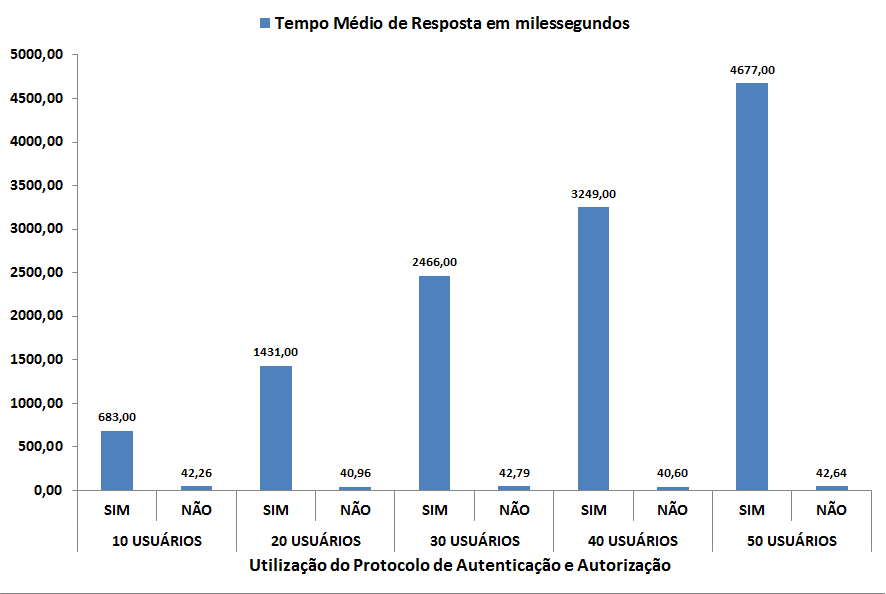
\includegraphics[width=1.0\textwidth]{grafico_teste_desempenho.png}
    \caption{Fluxo do protocolo de autenticação/autorização proposto, 1º cenário.}
    \label{fig:grafico_teste_desempenho}
\end{figure}


\section{Estudo de caso 2}\label{sec:caso2}

Os ambientes de teste utilizados foram o laboratório de informática da Universidade de Brasília e o da Divisão de Tecnologia da Policia Civil do Distrito Federal, uma vez que se busca resultados mais próximos da realidade hoje vivenciado pela PCDF.

Para a realização dos testes foram utilizadas configurações distintas de computadores, conforme apresentado na tabela~\ref{tb:estudo_caso2}.

Os web services adotados serão os mesmos definidos no estudo de caso 1, web service RESTfull de ocorrências criminais, que retornam informações gerais do sistema de ocorrências policiais.

\subsection{\emph{Configuração do ambiente de teste}}

Ambiente de teste foi o da Divisão de Tecnologia da Policia Civil do Distrito Federal, uma vez que se buscam resultados mais próximos da realidade hoje vivenciados pela PCDF.

Para a sua realização dos testes foram utilizados configurações distintas de computadores, conforme tabela abaixo. Essa configuração é idêntica a utilizada no estudo de caso 1.

%\begin{table}[!htpb]
%
%  \begin{tabular}{cp{13cm}}
\begin{table}[h]
    \begin{tabular}{|l|c|p{6cm}|}
    \hline
    \textbf{\emph{Máquina }}                   & \textbf{\emph{Quantidade}} & \textbf{\emph{Configuração}}                                                                               \\ \hline
    Servidor de Autenticação e Autorização  & 1          & Desktop DELL Intel Core I5-2450 2,5 GHz, 4 Gb RAM, 500 HD \\ \hline
    Servidor de Fachada REST  & 1          & Desktop DELL Intel Core I5-2450 2,5 GHz, 4 Gb RAM, 500 HD\\ \hline
    Cliente REST                   & 50        & Desktop DELL Intel Core I5-2450 2,5 GHz, 4 Gb RAM, 500 HD                                    \\ \hline
    \end{tabular}
    \caption {Ambiente de configuração estudo de caso 1}\label{tb:estudo_caso2}
\end{table}

Os servidores de Autenticação e Autorização, Fachada REST e Cliente REST, foram desenvolvidos utilizando a linguagem de programação funcional \emph{Haskell} acessando um banco de dados não relacional, \emph{Apache CouchDB}, conforme apresentado na seção~\ref{sec:implementacao}. O sistema operacional utilizado nessas máquinas foi o Linux Ubuntu 12.04 LTS-64 bits..

\subsection{\emph{Planejamento do experimento}}

O planejamento adotado neste estudo de caso procurou adaptar a realidade vivenciada na PCDF no oferecimento de um serviço. Desta forma, observou-se um cenário extremo de utilização, onde o número médio de requisições aos serviços RESTfull ofertados pela PCDF em 1 hora era de aproximadamente 1200 requisições, ou seja, uma média de duas requisições a cada segundo.

Sendo assim, objetiva-se verificar se o protocolo consegue atender um a caso extremo, que se assemelhe ao vivenciada pela PCDF. Logo, para simular esta situação, realizou-se um teste automatizado, utilizando a ferramenta Apache JMeter, que é um software open source, desenvolvido em Java.

Para realizar o experimento, a abordagem utilizada foi a da utilização de dois fatores: uso do protocolo de autenticação e autorização proposto (SIM/NÃO) e o número de usuários (50) com dois níveis e um nível respectivamente.  Para realizar o experimento foram realizadas 100 requisições para cada usuário, com um intervalo de 2 (dois) segundos de iniciação para cada usuário. As variáveis de resposta adotadas foram o tempo médio de resposta das requisições e a vazão média de requisições por segundo.

\subsection{Análise dos resultados}

A análise dos resultados obtidos com a execução do experimento ocorreu com a observação do tempo médio de resposta e com a verificação da vazão, número de requisições atendidas por segundo, que foi coletado ao final da execução do teste aplicado a um grupo de 50 usuários simultâneos. Dessa forma, foram coletadas 5000(cinco mil) amostras que utilizaram o protocolo de autenticação e autorização proposto em um período de 11 minutos. Os resultados estatísticos são apresentados na tabela~\ref{tb:estatistica_com_cripto_50}.

Em um cenário extremo, observou-se que a PCDF pode ter que responder a uma média de 1200 requisições de um serviço que fornece informações sobre ocorrências policiais em um período de 1 (uma) hora, ou seja, duas requisições a cada um segundo. Neste caso, os resultados obtidos com o experimento realizado com os 50 usuários simultâneos, demonstrou que o tempo médio de resposta foi de 4677 milessegundos ou aproximadamente 4,677 segundos e que a vazão média, que é o número de requisições atendidas por segundo, foi de 8,62 requisições por segundo. Ao se realizar a comparação deste cenário com o cenário extremo vivenciado pela PCDF, verificou-se que a arquitetura, do ponto de vista de vazão, atende perfeitamente o pior caso relatado, que é de 2 duas requisições por segundo. O que garante a qualidade do serviço ofertado pelo protocolo de autenticação e autorização proposto.

\begin{table}[h]
\centering
\begin{tabular}{|l|l|}
\hline
\textbf{Informação} & \textbf{Valor} \\ \hline
Nº de Requisições   &  5000              \\ \hline
Média               &  4677             \\ \hline
Mínimo              &  118          \\ \hline
Máximo              &  21665        \\ \hline
Desvio Padrão       &  3170,49      \\ \hline
\% Erro             &  0,0          \\ \hline
Vazão/seg           &  8,62     \\ \hline
Kbps                &  11,8         \\ \hline
Média de Bytes      &  1401,05      \\ \hline
\end{tabular}
\caption {Estatística básica com a utilização do protocolo de autenticação e autorização para 50 usuários.}\label{tb:estatistica_com_cripto_50}
\end{table}

\section{Síntese do capítulo}
Neste capítulo foram realizados dois estudos de caso, onde foram detalhados os cenários que seriam analisados, os ambientes e planejamento de testes e as referidas análises dos resultados obtidos.

Os estudos de casos realizados evidenciaram que o impacto no desempenho é significativo quando comparado com a não utilização da proposta. Porém os tempos médios obtidos estão dentro de um tempo médio esperado, que é abaixo de 5 segundos. Observou-se ainda, que em um cenário extremo de utilização, onde a PCDF tenha que atender a uma média de 2 duas requisições por segundo, e um período de 1 uma hora, ou seja 1200 requisições, a arquitetura proposta atende perfeitamente, pois consegue atender a 8,62 requisições por segundo em um cenário extremo onde foram realizados 5000 requisições em aproximadamente em 10 minutos.
